\section*{Anhang}\label{sec:anhang}
\begin{figure}[H]
    \centering
    \begin{subfigure}{0.45\textwidth}
        \centering
        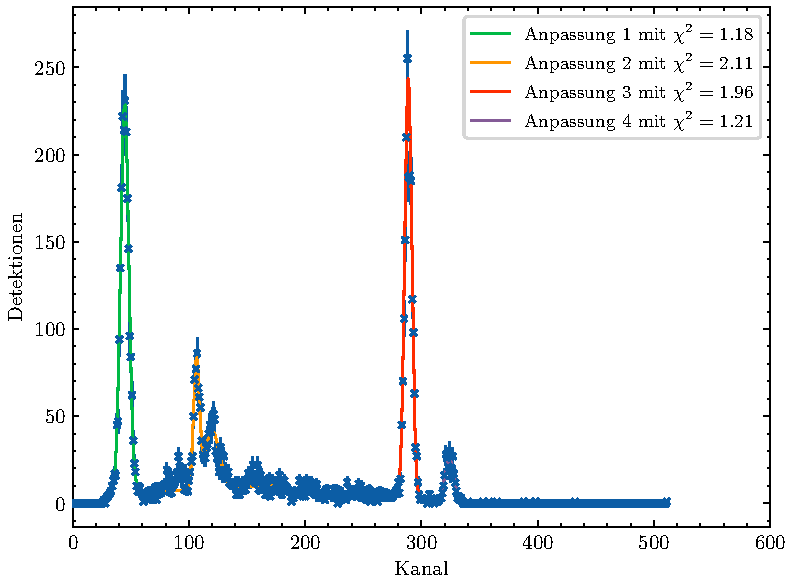
\includegraphics[width=\linewidth]{../figs/Ag}
        \caption{Silber}
    \end{subfigure}
    \begin{subfigure}{0.45\textwidth}
        \centering
        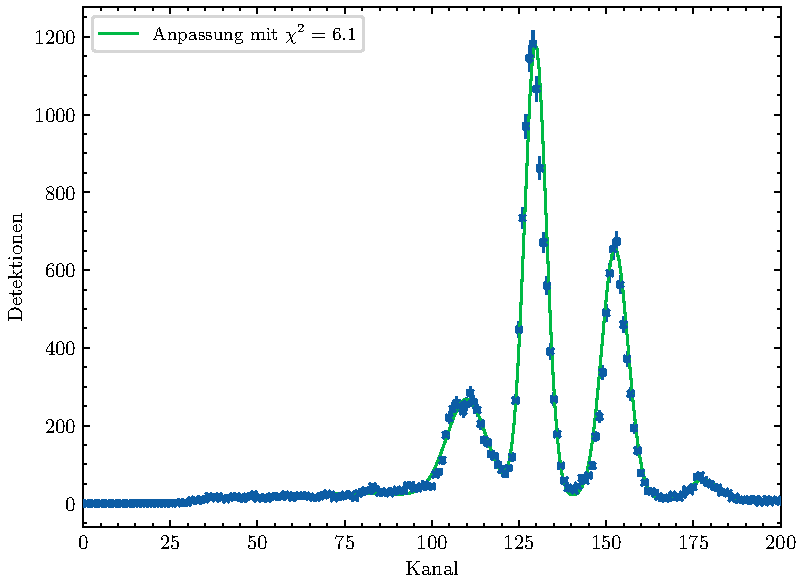
\includegraphics[width=\linewidth]{../figs/Au}
        \caption{Gold}
    \end{subfigure}
    \caption{Referenzspektren für Silber und Gold.}\label{fig:ag_au}
\end{figure}
\begin{figure}[H]
    \centering
    \begin{subfigure}{0.45\textwidth}
        \centering
        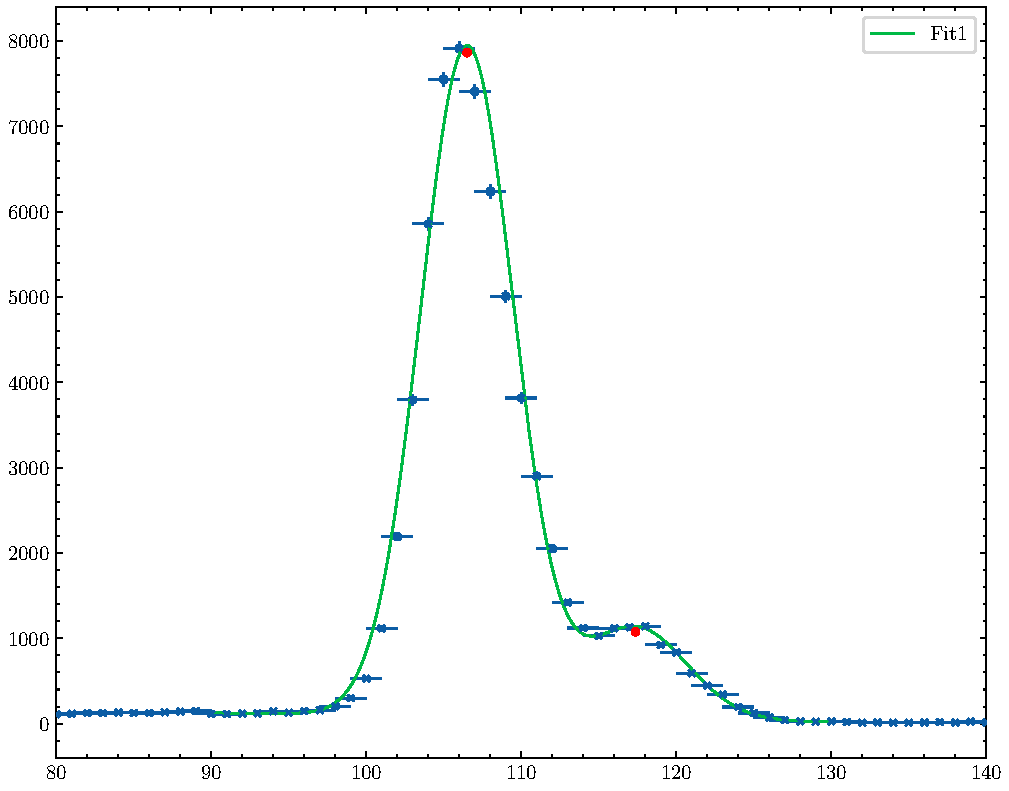
\includegraphics[width=\linewidth]{../figs/Cu}
        \caption{Kupfer}
    \end{subfigure}
    \begin{subfigure}{0.45\textwidth}
        \centering
        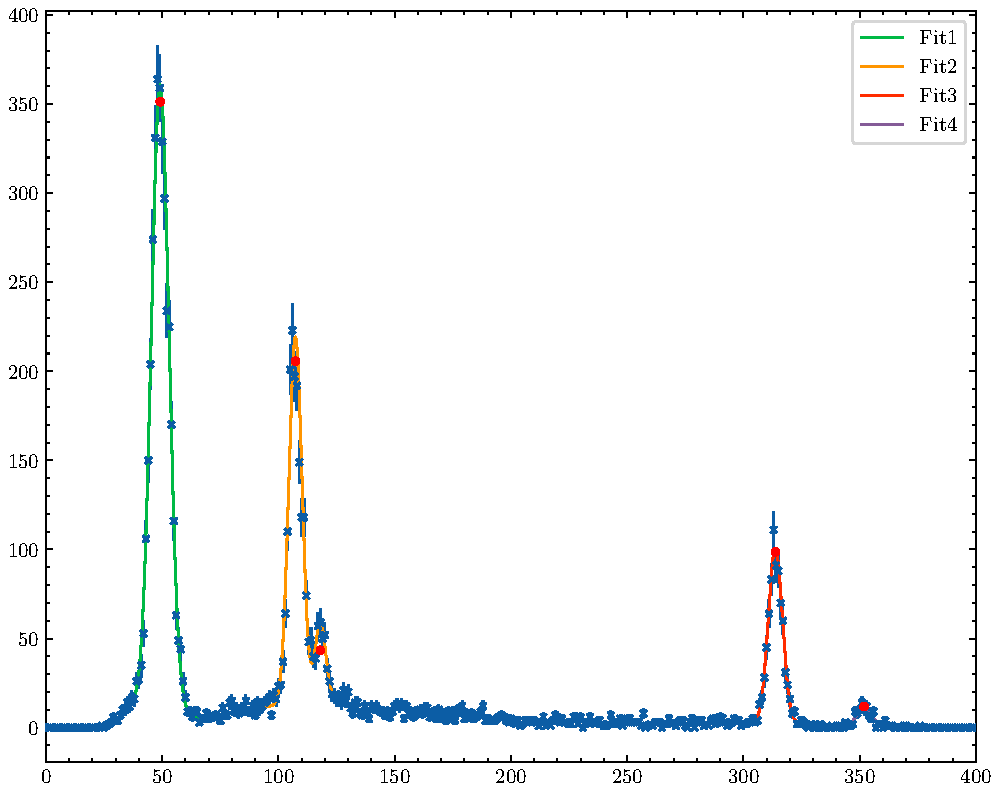
\includegraphics[width=\linewidth]{../figs/In}
        \caption{Indium}
    \end{subfigure}
    \caption{Referenzspektren für Kupfer und Indium.}\label{fig:cu_in}
\end{figure}
\begin{figure}[H]
    \centering
    \begin{subfigure}{0.45\textwidth}
        \centering
        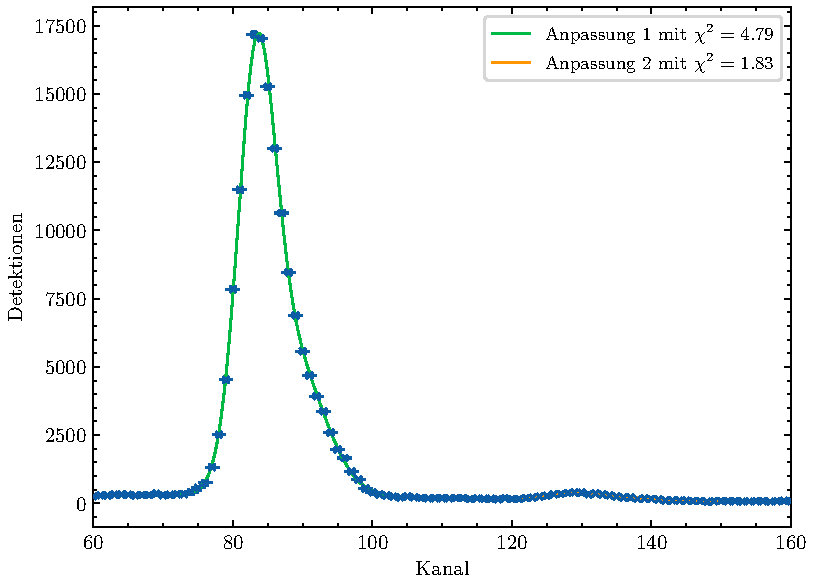
\includegraphics[width=\linewidth]{../figs/Fe}
        \caption{Eisen}
    \end{subfigure}
    \begin{subfigure}{0.45\textwidth}
        \centering
        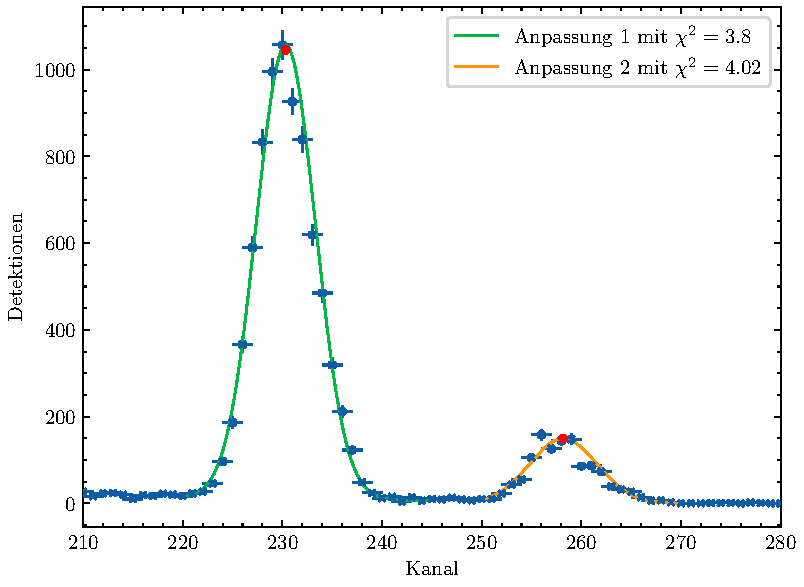
\includegraphics[width=\linewidth]{../figs/Mo}
        \caption{Molybdän}
    \end{subfigure}
    \caption{Referenzspektren für Eisen und Molybdän.}\label{fig:fe_mo}
\end{figure}
\begin{figure}[H]
    \centering
    \begin{subfigure}{0.45\textwidth}
        \centering
        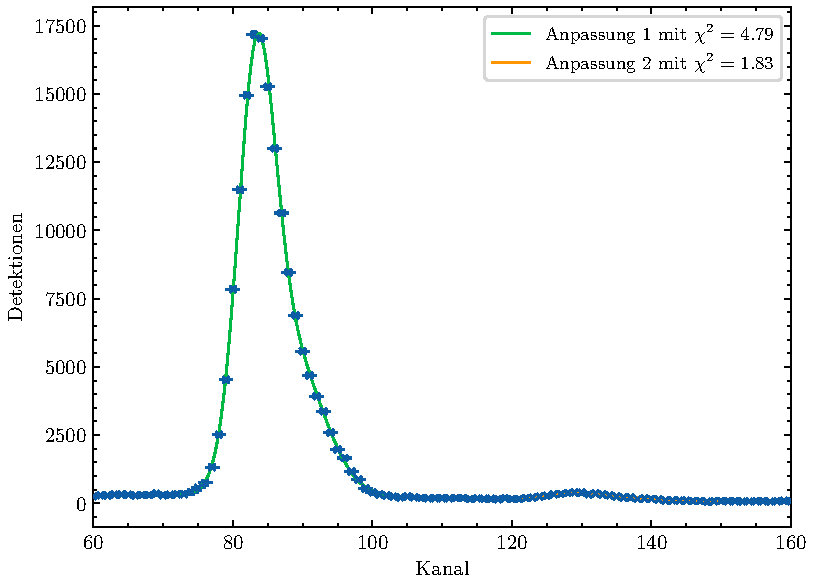
\includegraphics[width=\linewidth]{../figs/Fe}
        \caption{Nickel}
    \end{subfigure}
    \begin{subfigure}{0.45\textwidth}
        \centering
        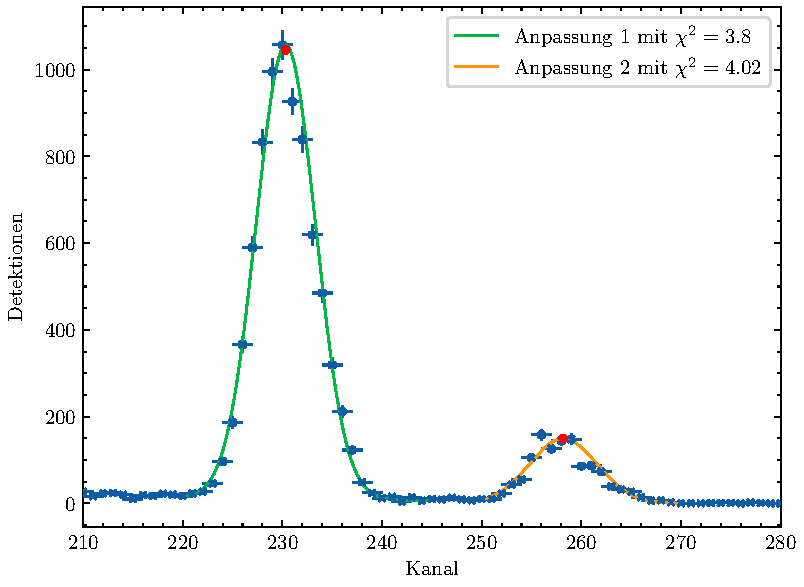
\includegraphics[width=\linewidth]{../figs/Mo}
        \caption{Blei}
    \end{subfigure}
    \caption{Referenzspektren für Nickel und Blei.}\label{fig:ni_pb}
\end{figure}
\begin{figure}[H]
    \centering
    \begin{subfigure}{0.45\textwidth}
        \centering
        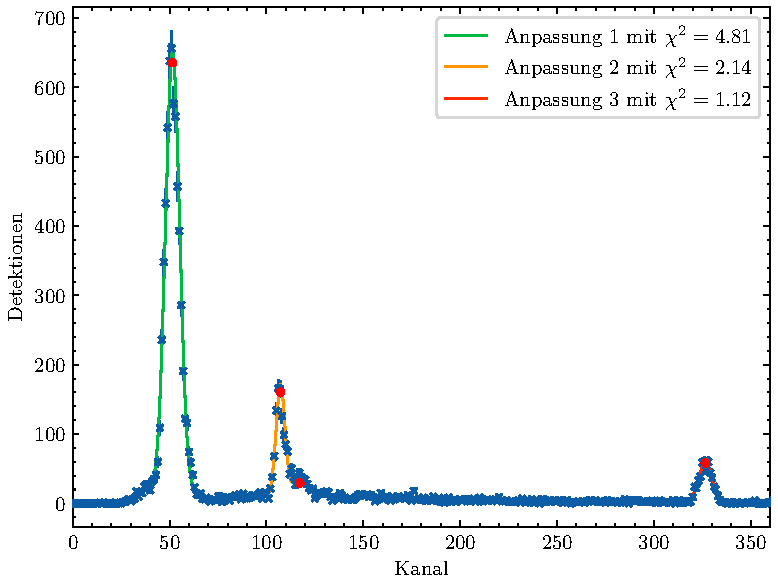
\includegraphics[width=\linewidth]{../figs/Sn}
        \caption{Zinn}
    \end{subfigure}
    \begin{subfigure}{0.45\textwidth}
        \centering
        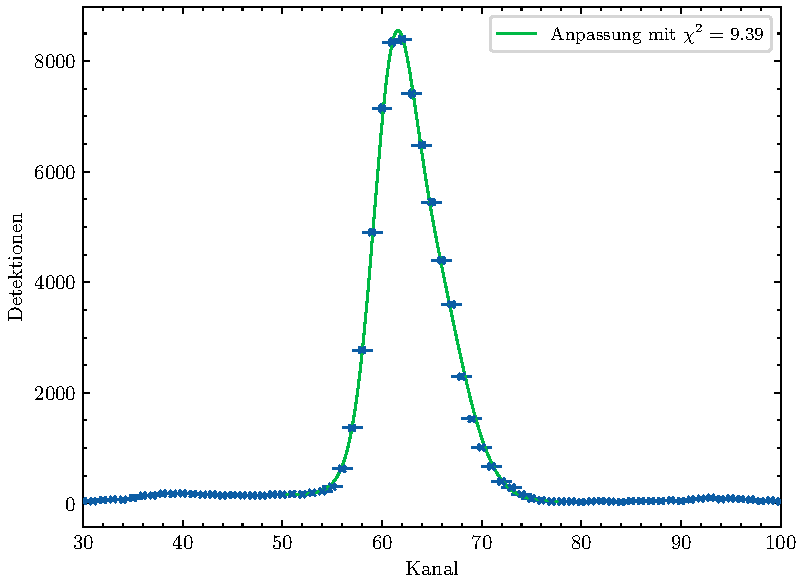
\includegraphics[width=\linewidth]{../figs/Titan}
        \caption{Titan}
    \end{subfigure}
    \caption{Referenzspektren für Zinn und Titan.}\label{fig:sn_ti}
\end{figure}
\begin{figure}[H]
    \centering
    \begin{subfigure}{0.45\textwidth}
        \centering
        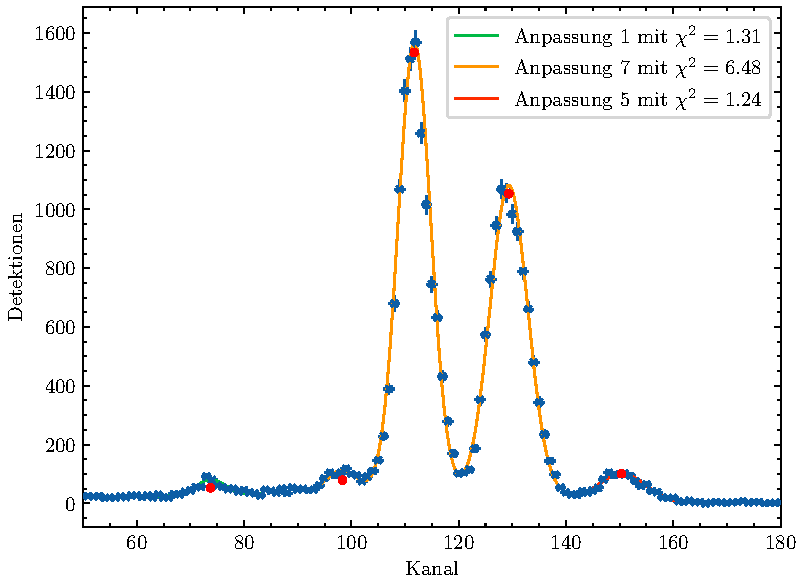
\includegraphics[width=\linewidth]{../figs/W}
        \caption{Wolfram}
    \end{subfigure}
    \begin{subfigure}{0.45\textwidth}
        \centering
        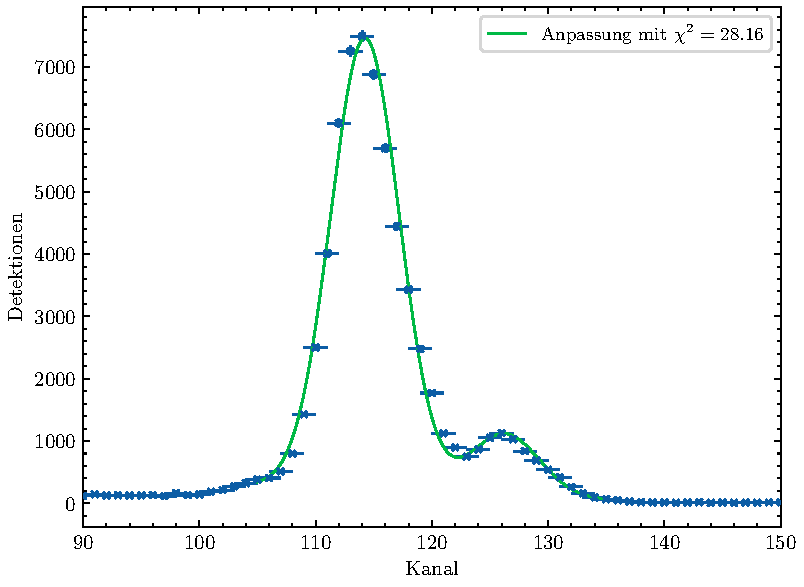
\includegraphics[width=\linewidth]{../figs/Zn}
        \caption{Zink}
    \end{subfigure}
    \caption{Referenzspektren für Wolfram und Zink.}\label{fig:w_zn}
\end{figure}
\begin{figure}[H]
	\centering
	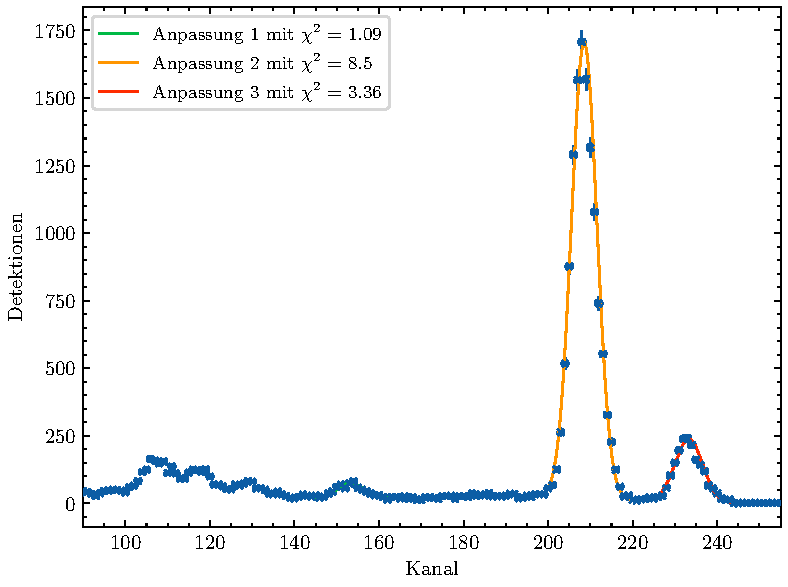
\includegraphics[width=0.6\linewidth]{../figs/Zr.pdf}
	\caption{Referenzspektrum für Zirconium.}
	\label{fig:zr}
\end{figure}